\documentclass{article}

\usepackage{tkz-euclide}

\begin{document}
    \begin{center}
        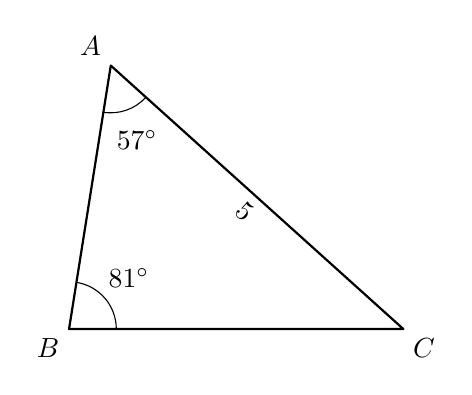
\begin{tikzpicture}
            \tkzDefPoints{0/0/O, 5/0/C}
            \tkzDefPointBy[rotation=center C angle 81+57-180](O)\tkzGetPoint{A}
            \tkzDefPointBy[rotation=center A angle -57](C)\tkzGetPoint{B1}
            \tkzInterLL(O,C)(A,B1)\tkzGetPoint{B}
            \tkzDrawPolygon[thick](A,B,C)
            \tkzMarkAngle[fill=gray, size=0.6](B,A,C)
            \tkzMarkAngle[size=0.6](C,B,A)
            \tkzLabelAngle(B,A,C){\(57^{\circ}\)}
            \tkzLabelAngle(C,B,A){\(81^{\circ}\)}
            \tkzLabelSegment[sloped](A,C){\(5\)}
            \tkzLabelPoint[above left](A){\(A\)}
            \tkzLabelPoint[below left](B){\(B\)}
            \tkzLabelPoint[below right](C){\(C\)}
        \end{tikzpicture}
    \end{center}
\end{document}